\documentclass{article}
\usepackage{graphicx} % Required for inserting images
\usepackage{amsmath}
\usepackage{amssymb} % used for math symbols
\usepackage{mathtools}
\usepackage{enumitem}
\usepackage{wasysym}
\usepackage{float}
\usepackage{minted}
\usepackage{tikz}


\title{Computer Grafik Blatt 9}
\date{June 2023}

\begin{document}

\maketitle

\section*{Aufgabe 1.}

\subsection*{(a)}
% draw points b_0 = (1,0), b_1 = (4,1), b_2 = (0,1), b_3 = (3,0) using tikz
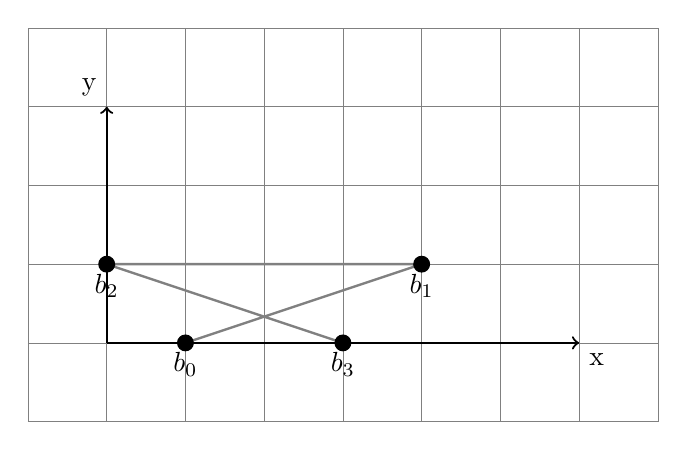
\begin{tikzpicture}
    \draw[step=1cm,gray,very thin] (-1,-1) grid (7,4);
    \draw[thick,->] (0,0) -- (6,0) node[anchor=north west] {x};
    \draw[thick,->] (0,0) -- (0,3) node[anchor=south east] {y};
    \draw[gray, line width=0.3mm] (1,0) -- (4,1) -- (0,1) -- (3,0);
    \draw[fill=black] (1,0) circle (0.1cm) node[anchor=north] {$b_0$};
    \draw[fill=black] (4,1) circle (0.1cm) node[anchor=north] {$b_1$};
    \draw[fill=black] (0,1) circle (0.1cm) node[anchor=north] {$b_2$};
    \draw[fill=black] (3,0) circle (0.1cm) node[anchor=north] {$b_3$};
\end{tikzpicture}

\subsection*{(b)}
Erster Schritt

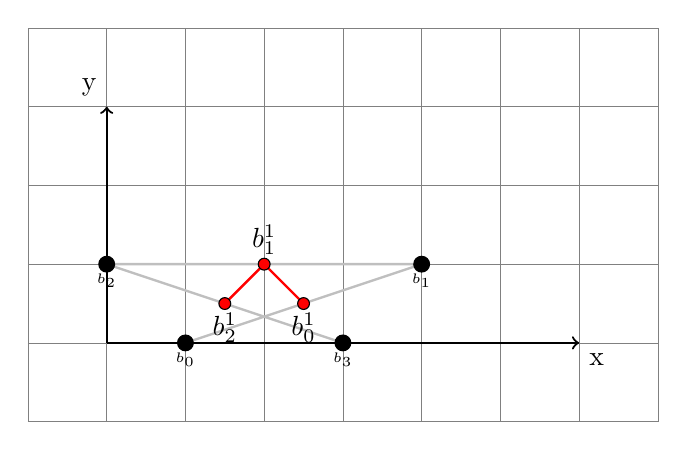
\begin{tikzpicture}
    \draw[step=1cm,gray,very thin] (-1,-1) grid (7,4);
    \draw[thick,->] (0,0) -- (6,0) node[anchor=north west] {x};
    \draw[thick,->] (0,0) -- (0,3) node[anchor=south east] {y};
    \draw[lightgray, line width=0.3mm] (1,0) -- (4,1) -- (0,1) -- (3,0);
    \draw[fill=black] (1,0) circle (0.1cm) node[anchor=north, font=\tiny] {$b_0$};
    \draw[fill=black] (4,1) circle (0.1cm) node[anchor=north, font=\tiny] {$b_1$};
    \draw[fill=black] (0,1) circle (0.1cm) node[anchor=north, font=\tiny] {$b_2$};
    \draw[fill=black] (3,0) circle (0.1cm) node[anchor=north, font=\tiny] {$b_3$};
    \draw[red, line width=0.3mm] (2.5,0.5) -- (2,1) -- (1.5,0.5);
    \draw[fill=red] (2.5,0.5) circle (0.075cm) node[anchor=north] {$b_{0}^{1}$};
    \draw[fill=red] (2,1) circle (0.075cm) node[anchor=south] {$b_{1}^{1}$};
    \draw[fill=red] (1.5,0.5) circle (0.075cm) node[anchor=north] {$b_{2}^{1}$};
\end{tikzpicture}

Zweiter Schritt

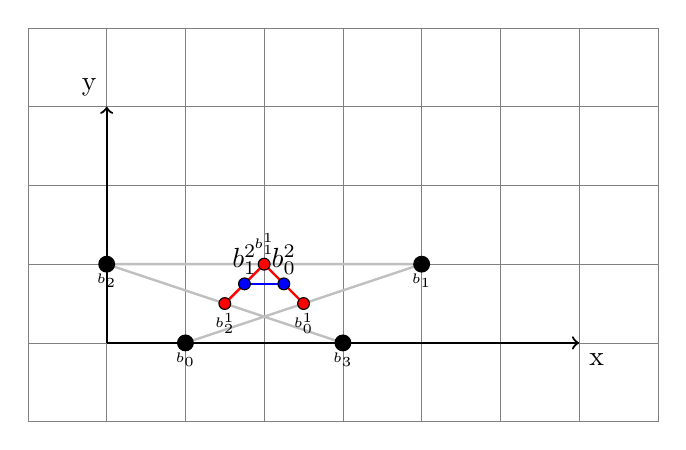
\begin{tikzpicture}
    \draw[step=1cm,gray,very thin] (-1,-1) grid (7,4);
    \draw[thick,->] (0,0) -- (6,0) node[anchor=north west] {x};
    \draw[thick,->] (0,0) -- (0,3) node[anchor=south east] {y};
    \draw[lightgray, line width=0.3mm] (1,0) -- (4,1) -- (0,1) -- (3,0);
    \draw[fill=black] (1,0) circle (0.1cm) node[anchor=north, font=\tiny] {$b_0$};
    \draw[fill=black] (4,1) circle (0.1cm) node[anchor=north, font=\tiny] {$b_1$};
    \draw[fill=black] (0,1) circle (0.1cm) node[anchor=north, font=\tiny] {$b_2$};
    \draw[fill=black] (3,0) circle (0.1cm) node[anchor=north, font=\tiny] {$b_3$};
    \draw[red, line width=0.3mm] (2.5,0.5) -- (2,1) -- (1.5,0.5);
    \draw[fill=red] (2.5,0.5) circle (0.075cm) node[anchor=north, font=\tiny] {$b_{0}^{1}$};
    \draw[fill=red] (2,1) circle (0.075cm) node[anchor=south, font=\tiny] {$b_{1}^{1}$};
    \draw[fill=red] (1.5,0.5) circle (0.075cm) node[anchor=north, font=\tiny] {$b_{2}^{1}$};
    \draw[blue, line width=0.3mm] (2.25,0.75) -- (1.75,0.75);
    \draw[fill=blue] (2.25,0.75) circle (0.075cm) node[anchor=south] {$b_{0}^{2}$};
    \draw[fill=blue] (1.75,0.75) circle (0.075cm) node[anchor=south] {$b_{1}^{2}$};
\end{tikzpicture}

Letzter Schritt

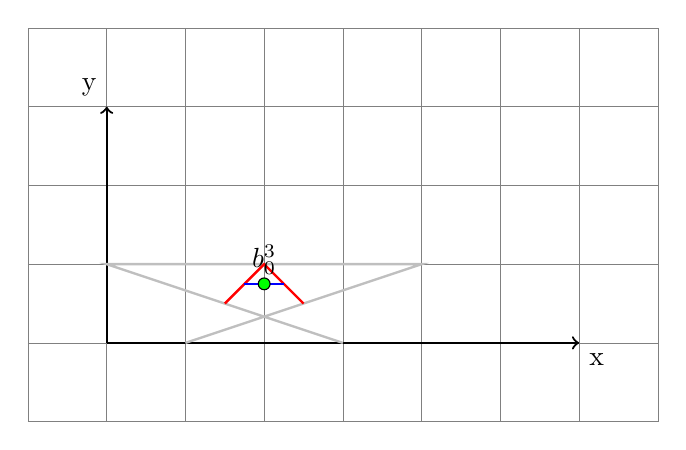
\begin{tikzpicture}
    \draw[step=1cm,gray,very thin] (-1,-1) grid (7,4);
    \draw[thick,->] (0,0) -- (6,0) node[anchor=north west] {x};
    \draw[thick,->] (0,0) -- (0,3) node[anchor=south east] {y};
    \draw[lightgray, line width=0.3mm] (1,0) -- (4,1) -- (0,1) -- (3,0);
    % \draw[fill=black] (1,0) circle (0.1cm) node[anchor=north, font=\tiny] {$b_0$};
    % \draw[fill=black] (4,1) circle (0.1cm) node[anchor=north, font=\tiny] {$b_1$};
    % \draw[fill=black] (0,1) circle (0.1cm) node[anchor=north, font=\tiny] {$b_2$};
    % \draw[fill=black] (3,0) circle (0.1cm) node[anchor=north, font=\tiny] {$b_3$};
    \draw[red, line width=0.3mm] (2.5,0.5) -- (2,1) -- (1.5,0.5);
    % \draw[fill=red] (2.5,0.5) circle (0.075cm) node[anchor=north, font=\tiny] {$b_{0}^{1}$};
    % \draw[fill=red] (2,1) circle (0.075cm) node[anchor=south, font=\tiny] {$b_{1}^{1}$};
    % \draw[fill=red] (1.5,0.5) circle (0.075cm) node[anchor=north, font=\tiny] {$b_{2}^{1}$};
    \draw[blue, line width=0.3mm] (2.25,0.75) -- (1.75,0.75);
    % \draw[fill=blue] (2.25,0.75) circle (0.075cm) node[anchor=south, font=\tiny] {$b_{0}^{2}$};
    % \draw[fill=blue] (1.75,0.75) circle (0.075cm) node[anchor=south, font=\tiny] {$b_{1}^{2}$};
    \draw[green, line width=0.3mm] (2,0.75);
    \draw[fill=green] (2,0.75) circle (0.075cm) node[anchor=south] {$b_{0}^{3}$};
\end{tikzpicture}

\subsection*{(c)}
Erster Schritt

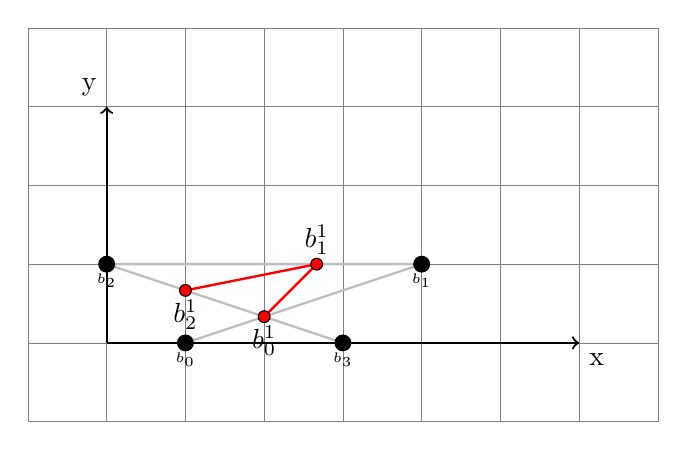
\begin{tikzpicture}
    \draw[step=1cm,gray,very thin] (-1,-1) grid (7,4);
    \draw[thick,->] (0,0) -- (6,0) node[anchor=north west] {x};
    \draw[thick,->] (0,0) -- (0,3) node[anchor=south east] {y};
    \draw[lightgray, line width=0.3mm] (1,0) -- (4,1) -- (0,1) -- (3,0);
    \draw[fill=black] (1,0) circle (0.1cm) node[anchor=north, font=\tiny] {$b_0$};
    \draw[fill=black] (4,1) circle (0.1cm) node[anchor=north, font=\tiny] {$b_1$};
    \draw[fill=black] (0,1) circle (0.1cm) node[anchor=north, font=\tiny] {$b_2$};
    \draw[fill=black] (3,0) circle (0.1cm) node[anchor=north, font=\tiny] {$b_3$};
    \draw[red, line width=0.3mm] (2,1/3) -- (8/3,1) -- (1,2/3);
    \draw[fill=red] (2,1/3) circle (0.075cm) node[anchor=north] {$b_{0}^{1}$};
    \draw[fill=red] (8/3,1) circle (0.075cm) node[anchor=south] {$b_{1}^{1}$};
    \draw[fill=red] (1,2/3) circle (0.075cm) node[anchor=north] {$b_{2}^{1}$};
\end{tikzpicture}

Zweiter Schritt

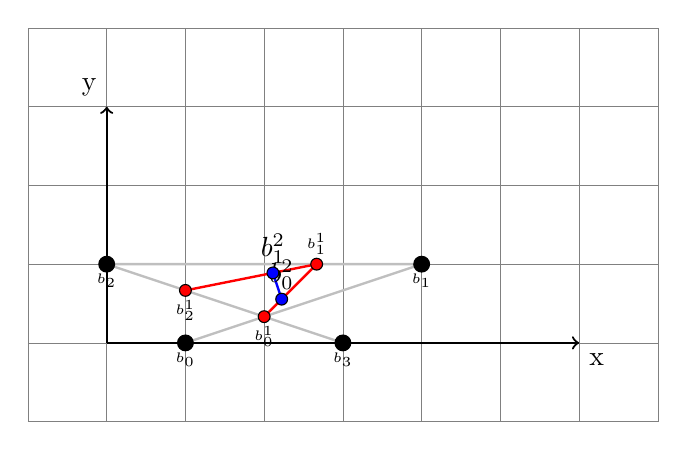
\begin{tikzpicture}
    \draw[step=1cm,gray,very thin] (-1,-1) grid (7,4);
    \draw[thick,->] (0,0) -- (6,0) node[anchor=north west] {x};
    \draw[thick,->] (0,0) -- (0,3) node[anchor=south east] {y};
    \draw[lightgray, line width=0.3mm] (1,0) -- (4,1) -- (0,1) -- (3,0);
    \draw[fill=black] (1,0) circle (0.1cm) node[anchor=north, font=\tiny] {$b_0$};
    \draw[fill=black] (4,1) circle (0.1cm) node[anchor=north, font=\tiny] {$b_1$};
    \draw[fill=black] (0,1) circle (0.1cm) node[anchor=north, font=\tiny] {$b_2$};
    \draw[fill=black] (3,0) circle (0.1cm) node[anchor=north, font=\tiny] {$b_3$};
    \draw[red, line width=0.3mm] (2,1/3) -- (8/3,1) -- (1,2/3);
    \draw[fill=red] (2,1/3) circle (0.075cm) node[anchor=north, font=\tiny] {$b_{0}^{1}$};
    \draw[fill=red] (8/3,1) circle (0.075cm) node[anchor=south, font=\tiny] {$b_{1}^{1}$};
    \draw[fill=red] (1,2/3) circle (0.075cm) node[anchor=north, font=\tiny] {$b_{2}^{1}$};
    \draw[blue, line width=0.3mm] (20/9,5/9) -- (19/9,8/9);
    \draw[fill=blue] (20/9,5/9) circle (0.075cm) node[anchor=south] {$b_{0}^{2}$};
    \draw[fill=blue] (19/9,8/9) circle (0.075cm) node[anchor=south] {$b_{1}^{2}$};
\end{tikzpicture}


Letzter Schritt

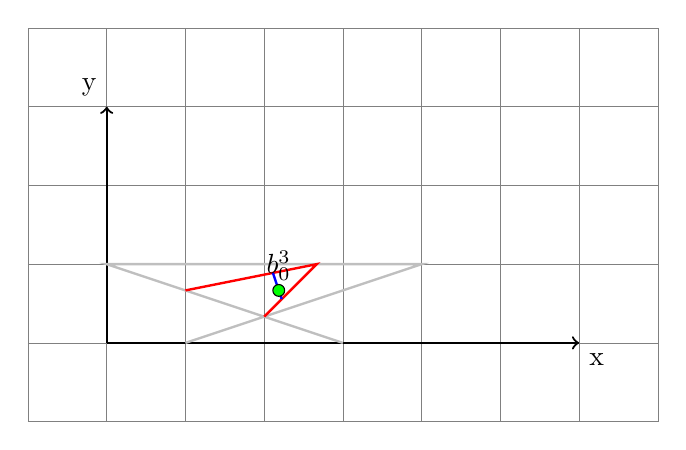
\begin{tikzpicture}
    \draw[step=1cm,gray,very thin] (-1,-1) grid (7,4);
    \draw[thick,->] (0,0) -- (6,0) node[anchor=north west] {x};
    \draw[thick,->] (0,0) -- (0,3) node[anchor=south east] {y};
    \draw[lightgray, line width=0.3mm] (1,0) -- (4,1) -- (0,1) -- (3,0);
    % \draw[fill=black] (1,0) circle (0.1cm) node[anchor=north, font=\tiny] {$b_0$};
    % \draw[fill=black] (4,1) circle (0.1cm) node[anchor=north, font=\tiny] {$b_1$};
    % \draw[fill=black] (0,1) circle (0.1cm) node[anchor=north, font=\tiny] {$b_2$};
    % \draw[fill=black] (3,0) circle (0.1cm) node[anchor=north, font=\tiny] {$b_3$};
    \draw[red, line width=0.3mm] (2,1/3) -- (8/3,1) -- (1,2/3);
    % \draw[fill=red] (2,1/3) circle (0.075cm) node[anchor=north, font=\tiny] {$b_{0}^{1}$};
    % \draw[fill=red] (8/3,1) circle (0.075cm) node[anchor=south, font=\tiny] {$b_{1}^{1}$};
    % \draw[fill=red] (1,2/3) circle (0.075cm) node[anchor=north, font=\tiny] {$b_{2}^{1}$};
    \draw[blue, line width=0.3mm] (20/9,5/9) -- (19/9,8/9);
    % \draw[fill=blue] (20/9,5/9) circle (0.075cm) node[anchor=south] {$b_{0}^{2}$};
    % \draw[fill=blue] (19/9,8/9) circle (0.075cm) node[anchor=south] {$b_{1}^{2}$};
    \draw[green, line width=0.3mm] (59/27, 2/3);
    \draw[fill=green] (59/27, 2/3) circle (0.075cm) node[anchor=south] {$b_{0}^{3}$};
\end{tikzpicture}

\subsection*{(d)}
\[
    \begin{aligned}
        b_{0}^{1} &= \frac{3}{4} b_{0} + \frac{1}{4} b_{1} \\
        &= \frac{3}{4} \cdot (1,0)^T + \frac{1}{4} \cdot (4,1)^T \\
        &= \left(\frac{7}{4}, \frac{1}{4}\right)^T \\
        & \\
        b_{1}^{1} &= \frac{3}{4} b_{1} + \frac{1}{4} b_{2} \\
        &= \frac{3}{4} \cdot (4,1)^T + \frac{1}{4} \cdot (0,1)^T \\
        &= \left(3,1\right)^T \\
        & \\
        b_{2}^{1} &= \frac{3}{4} b_{2} + \frac{1}{4} b_{3} \\
        &= \frac{3}{4} \cdot (0,1)^T + \frac{1}{4} \cdot (3,0)^T \\
        &= \left(\frac{3}{4}, 1\right)^T
    \end{aligned}
\]
\\
\\
\\
\\
\[
    \begin{aligned}
        b_{1}^{2} &= \frac{3}{4} b_{0}^{1} + \frac{1}{4} b_{1}^{1} \\
        &= \frac{3}{4} \cdot \left(\frac{7}{4}, \frac{1}{4}\right)^T + \frac{1}{4} \cdot \left(3,1\right)^T \\
        &= \left(\frac{33}{16}, \frac{7}{16}\right)^T \\
        & \\
        b_{2}^{2} &= \frac{3}{4} b_{1}^{1} + \frac{1}{4} b_{2}^{1} \\
        &= \frac{3}{4} \cdot \left(3,1\right)^T + \frac{1}{4} \cdot \left(\frac{3}{4}, 1\right)^T \\
        &= \left(\frac{39}{16}, 1\right)^T
    \end{aligned}
\]
\\
\\
\\
\\
\[
    \begin{aligned}
        b_{0}^{3} &= \frac{3}{4} b_{0}^{2} + \frac{1}{4} b_{1}^{2} \\
        &= \frac{3}{4} \cdot \left(\frac{33}{16}, \frac{7}{16}\right)^T + \frac{1}{4} \cdot \left(\frac{39}{16}, 1\right)^T \\
        &= \left(\frac{69}{32}, \frac{37}{64}\right)^T
    \end{aligned}
\]

\subsection*{(e)}



\subsection*{(f)}

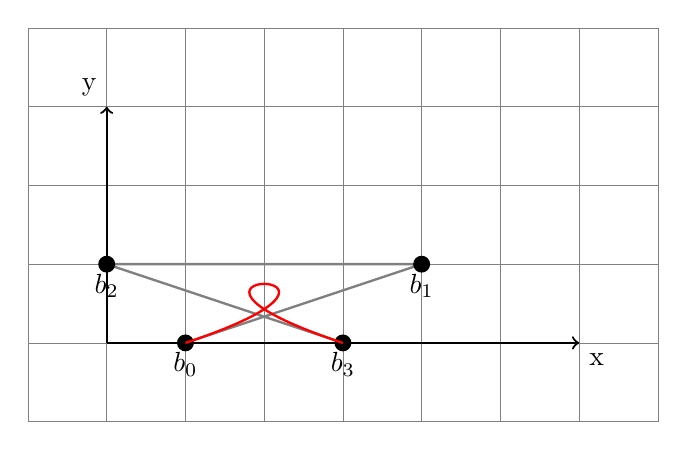
\begin{tikzpicture}
    \draw[step=1cm,gray,very thin] (-1,-1) grid (7,4);
    \draw[thick,->] (0,0) -- (6,0) node[anchor=north west] {x};
    \draw[thick,->] (0,0) -- (0,3) node[anchor=south east] {y};
    \draw[gray, line width=0.3mm] (1,0) -- (4,1) -- (0,1) -- (3,0);
    \draw[fill=black] (1,0) circle (0.1cm) node[anchor=north] {$b_0$};
    \draw[fill=black] (4,1) circle (0.1cm) node[anchor=north] {$b_1$};
    \draw[fill=black] (0,1) circle (0.1cm) node[anchor=north] {$b_2$};
    \draw[fill=black] (3,0) circle (0.1cm) node[anchor=north] {$b_3$};
    \draw[red, line width=0.3mm] (1,0) .. controls (4,1) and (0,1) .. (3,0);
\end{tikzpicture}



\subsection*{(g)}
\[
    \begin{aligned}
        b_{0}^{1} &= \frac{1}{3} \cdot b_{0} + \frac{2}{3} \cdot b_{1} \\
        &= \frac{1}{3} \cdot (1,2,3,4)^T + \frac{2}{3} \cdot (1,3,3,7)^T \\
        &= \left(1,\frac{8}{3},3,6\right)^T
    \end{aligned}    
\]

\subsection*{(h)}



\end{document}